\section{Data}
%
  \begin{figure}
    \centering
    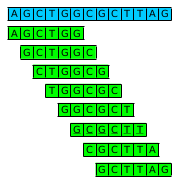
\includegraphics[scale=1]{kmers}
    \caption{%
      6-mer \textit{"word"} list production from original sequence.
    }
    \label{fig:kmers}
  \end{figure}
%
\subsection{Source}

The data for this project came from a Kaggle notebook, \textit{DNA Sequencing with Machine Learning}\footnote{\url{https://www.kaggle.com/code/nageshsingh/demystify-dna-sequencing-with-machine-learning/data}}.
%
DNA Coding Sequences are mostly comprised of exons and, in this corpus, range in length from  $\sim$1000 to $\sim$3,500 bases.

\subsection{Labeling}
Each sequence in the corpus of sequence data was annotated with one of seven Gene Families.  The Gene Family annotation was translated into an integer class label \textit{c} in $\{1, 2, 3, 4, 5, 6, 7\}$


\subsection{Preprocessing: Sequence to K-mer List}
%
The nucleotide bases comprise an \textit{alphabet} of the four letters \textit{b} in $\{A, G, C, T\}$.  A \textit{K-mer} is a \textit{k}-letter word comprised from \textit{letters} of this \textit{alphabet}.  Here we let \textit{k=6}.  The \textit{dictionary} contains up to $4^{6}$ \textit{words}, each 6 letters in length.\footnote{Dictionary size calculated as $alphabetSize^{wordLength}$ $\Rightarrow$ $4^{6}$ $\Rightarrow$ 4,096 words.}

\autoref{fig:kmers} above depicts 6bp \textit{"words"} derived from a sequence from the original corpus.  From this point on, all vectorization is based on a corpus of lists of \textit{6-mer "words"} rather than the original sequences.
%
